\section{Implementation of a point-to-point communication between a moving train and a station}

For this preliminary work, two network simulators were evaluated: the NS-3 and the OMNeT++. The approach of performing the evaluation of two network simulators allows, at this planning stage, to increase the knowledge on such simulators.

Figure \ref{fig:5.porto-caide} presents the train mobility model of the case-study: Porto-Caíde railway line operated by \textit{Comboios de Portugal} (CP). On this case-study, the simulator receives the \ac{GPS} coordinates of the line path and generates the mobility model. In addition, the train velocity is constant, without having in consideration the train stopping in stations. Future work will consider the velocity curves presented in subsection \ref{subs:353}: \textit{"Eco-driving – driving assistant"}.


\begin{figure}[h!]
	\centering
	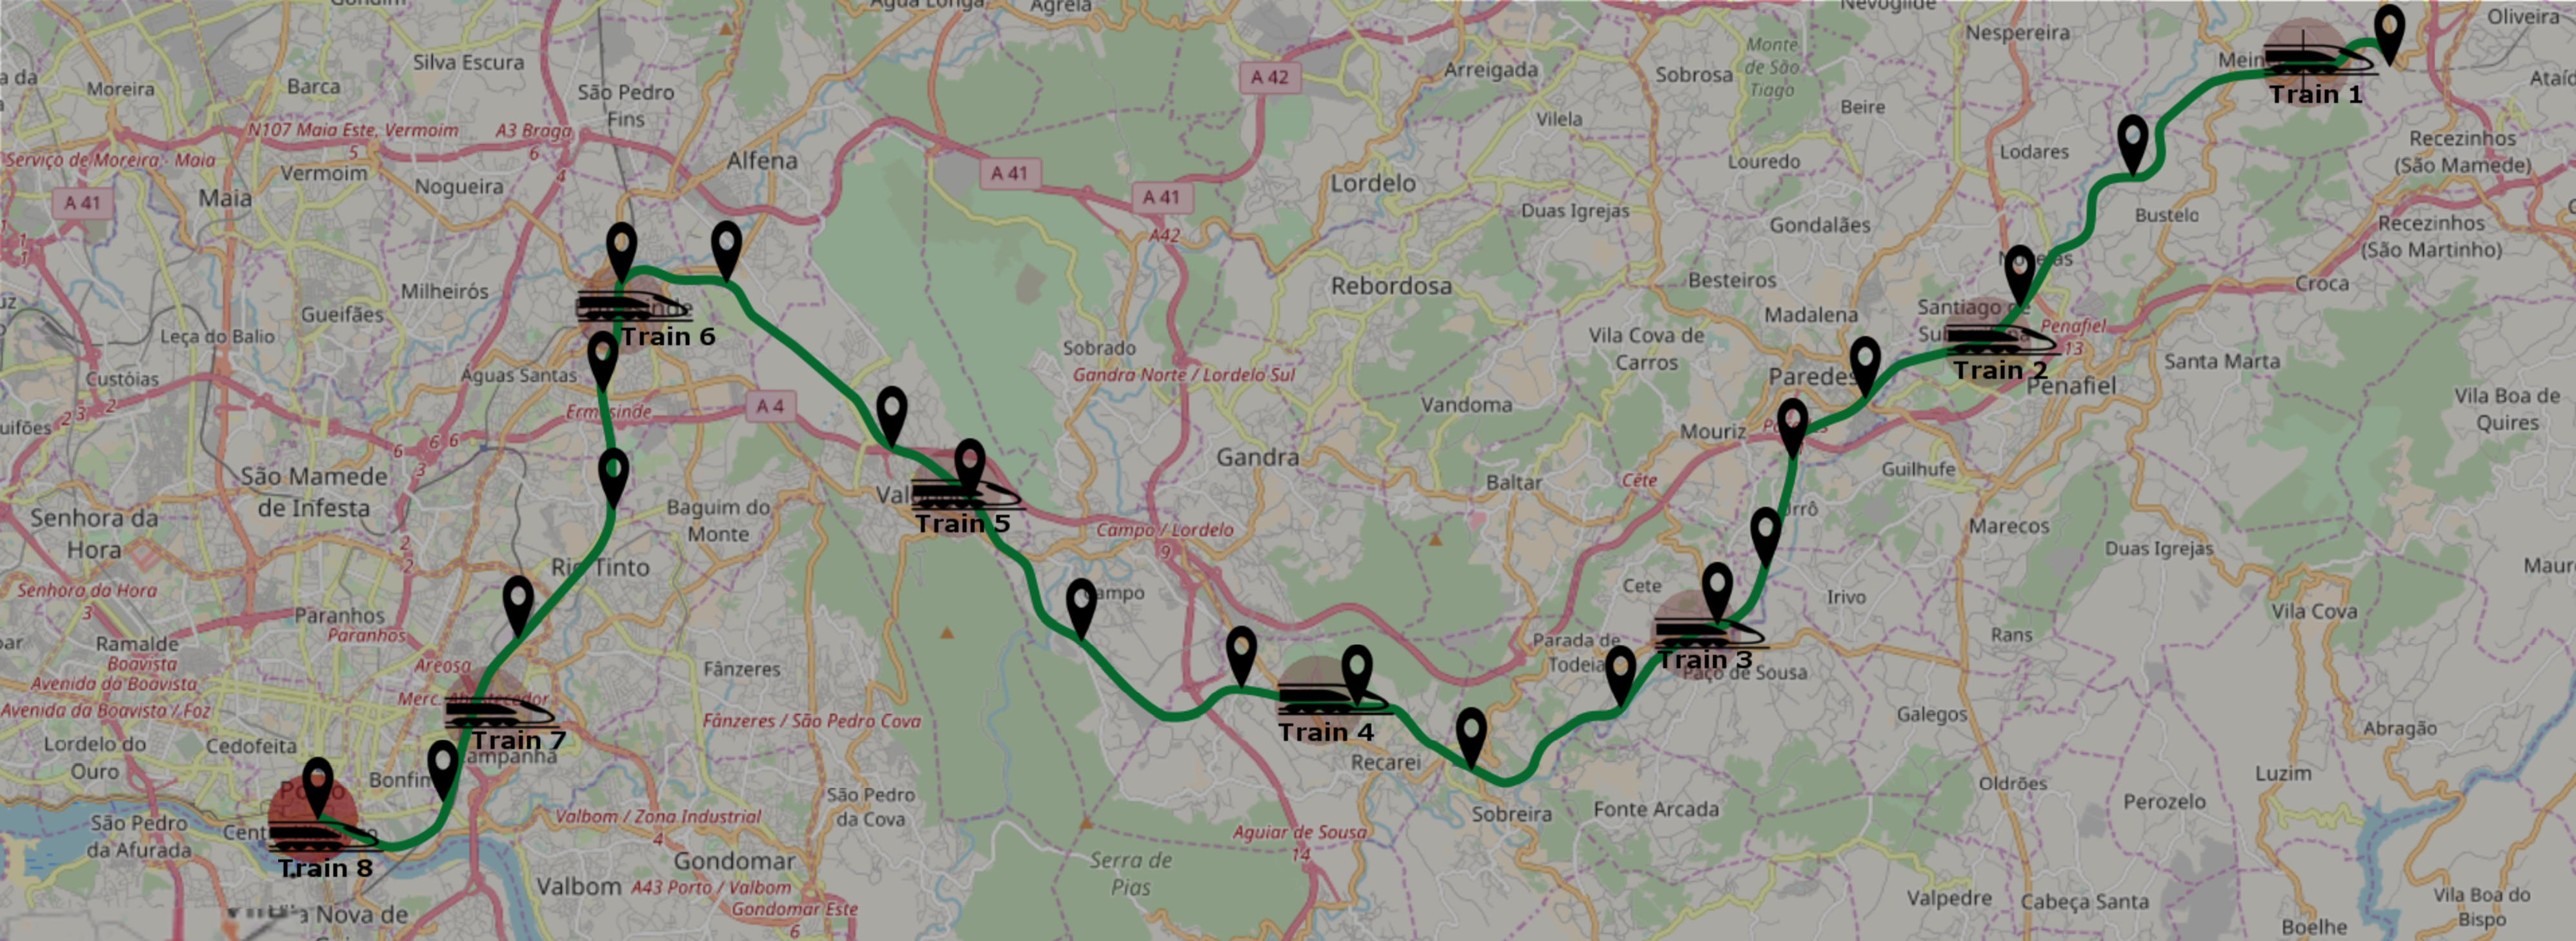
\includegraphics[width=\textwidth,keepaspectratio]{figures/50.PreliminaryW/porto-caide2}
	\caption{Porto-Caíde railway line: simulation using OMNeT++ network simulator.}
	\label{fig:5.porto-caide}
\end{figure}


The output of this mobility model will be, in the future, a file with the distances of each communication link, for each time-stamp. In this scope, each communication link will be the distance between each train and each of the train stations.

This output of the mobility model will be used by the network simulator to perform the simulation of the network link, that have this variable distance. To perform such simulation, the work of Noori and Valkama (2013) using the OMNeT++ simulator supports a vehicle communication with 802.11p standard, \cite{noori2013}. However, in this preliminary work, the NS-3 network simulator was tested. Figure \ref{fig:5.omnetpp+ns3} illustrate the interaction of both software simulators.

\begin{figure}[h!]
	\centering
	%	\vspace{-1em}
	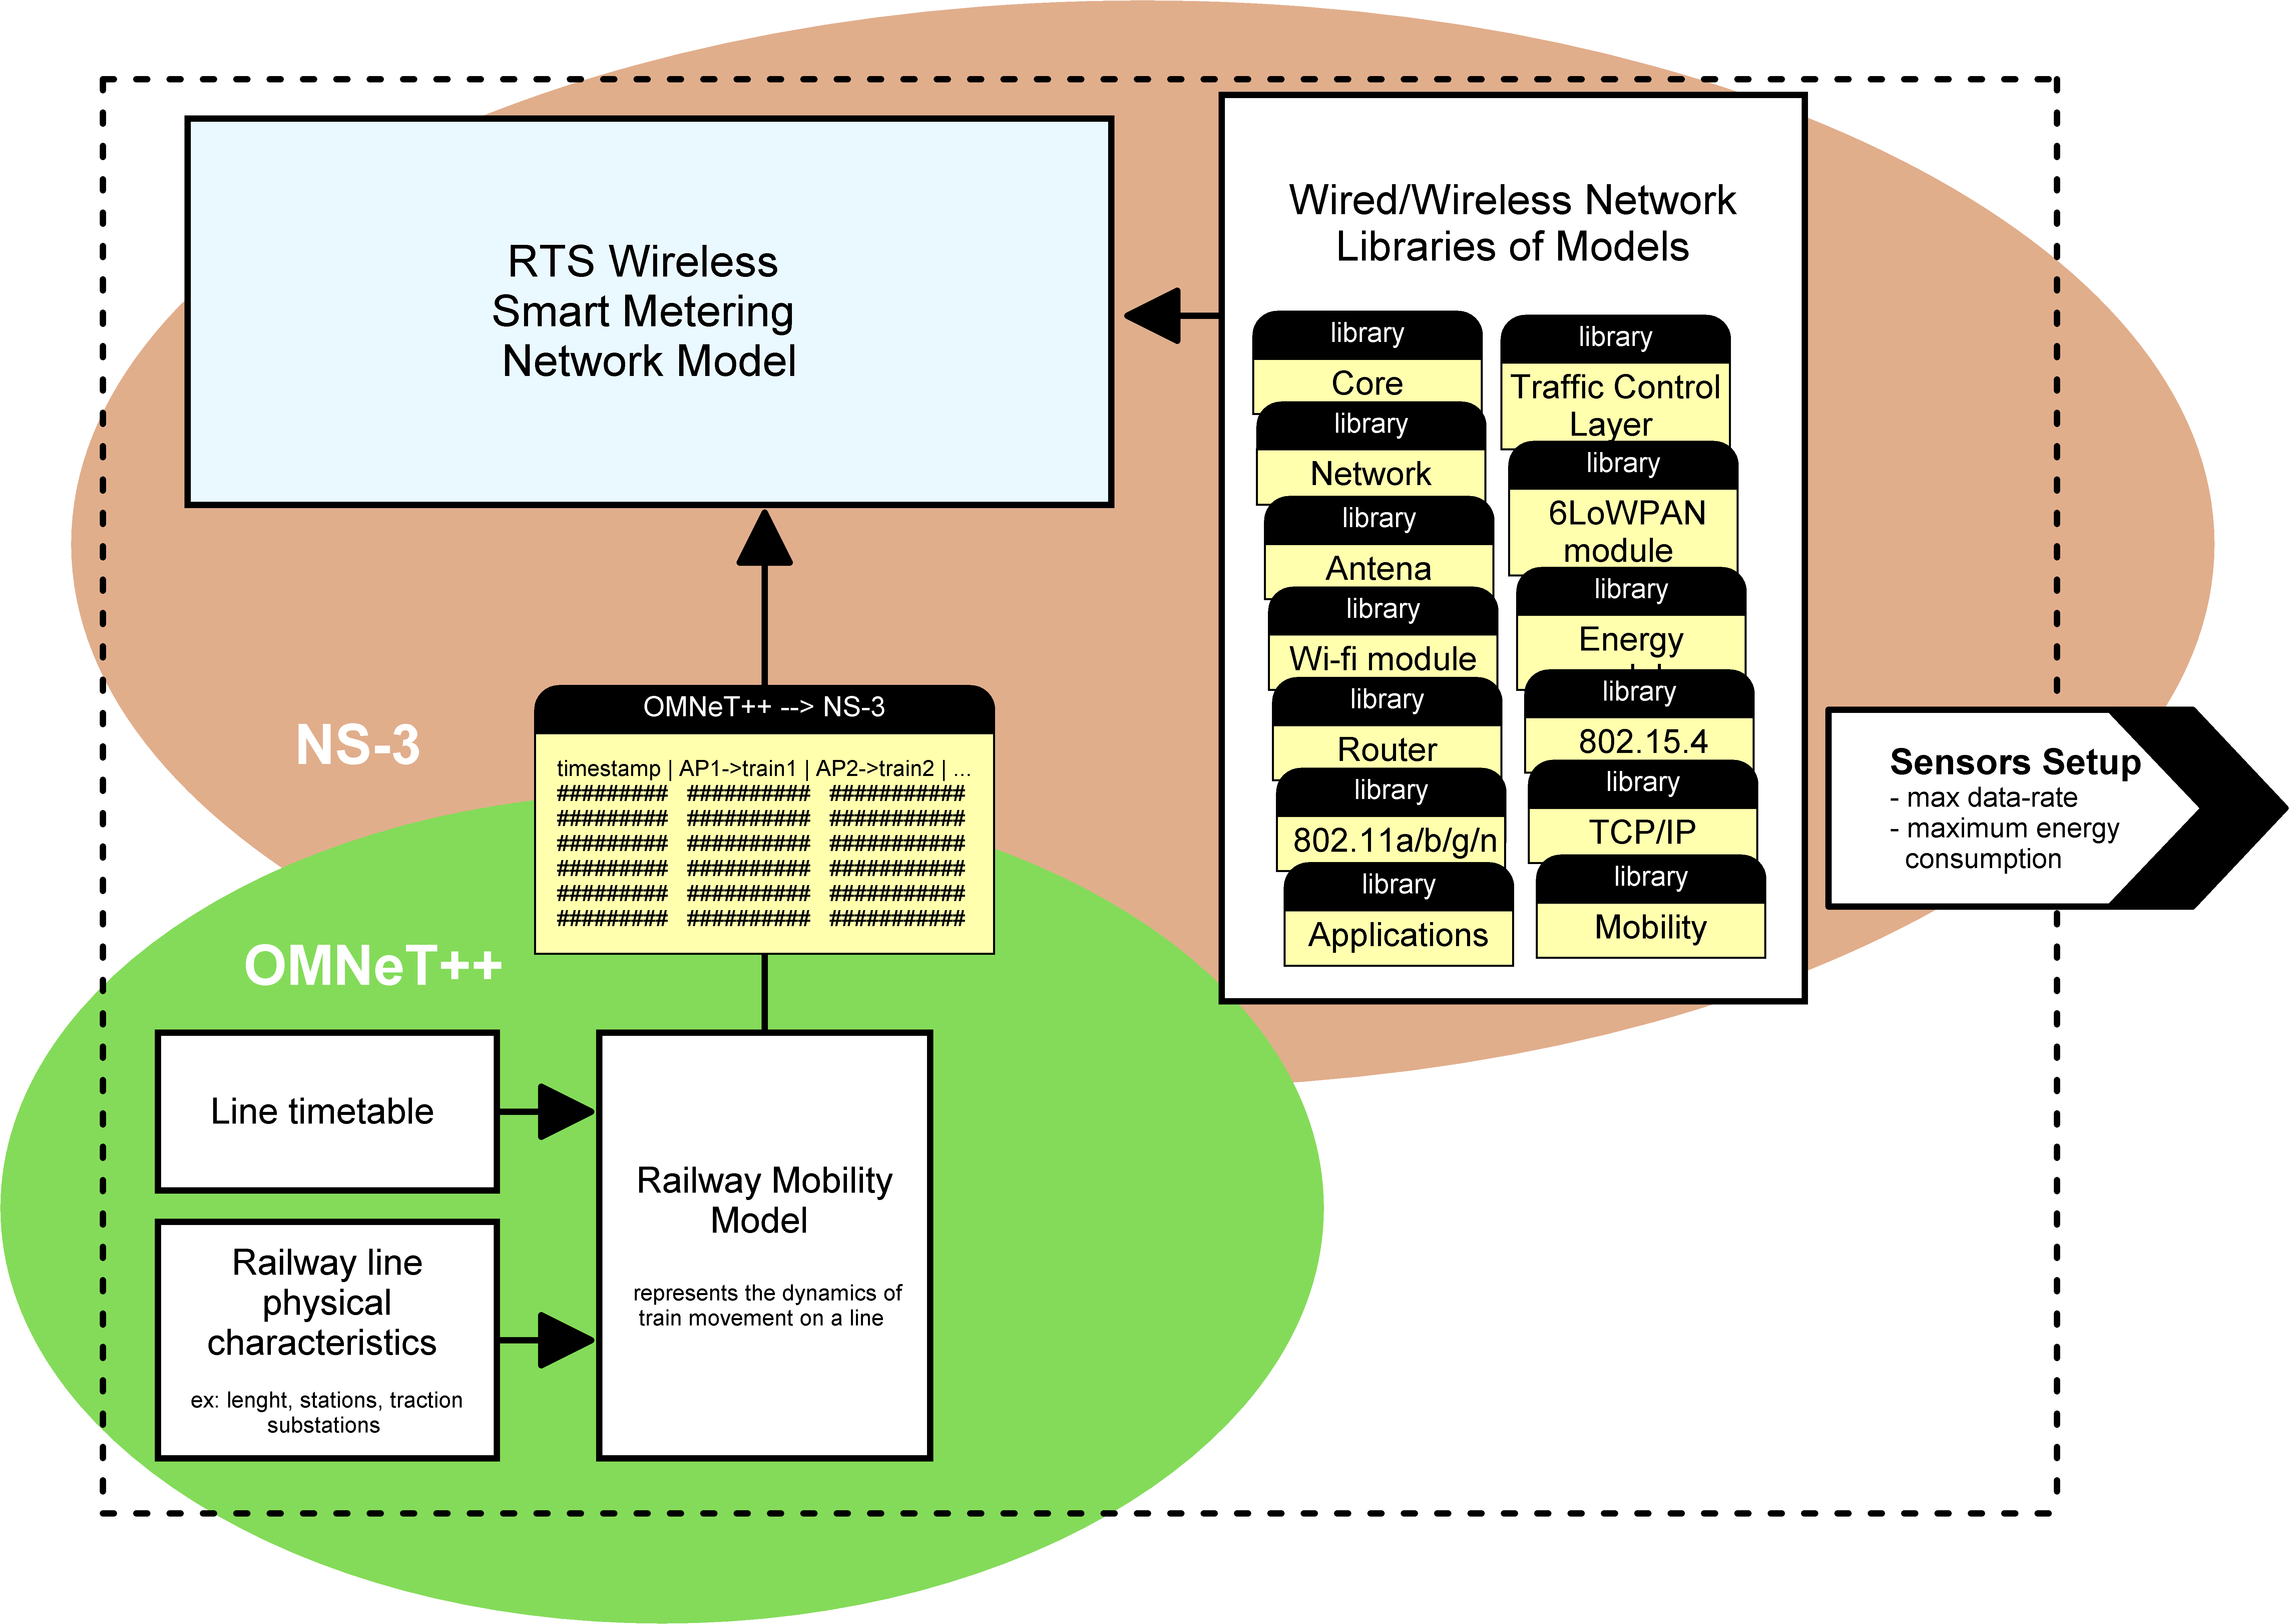
\includegraphics[width=0.85\textwidth,keepaspectratio]{figures/50.PreliminaryW/omnetpp+ns32}
	\caption{Simulator layers: proposed solution using OMNeT++ and NS-3.}
	\label{fig:5.omnetpp+ns3}
	%		\vspace{-2em}
\end{figure}

The simulation case-study for the NS-3 simulator was defined as a moving node at constant speed of 1 m/s that crosses a stationary node. In figure \ref{fig:5.distance-rate} is illustrated the different data-rates of different  802.11 network standards for the moving node that starts 200 meters away from the stationary node, crosses it and stops 200 meters away.

\begin{figure}[h!]
	\centering
	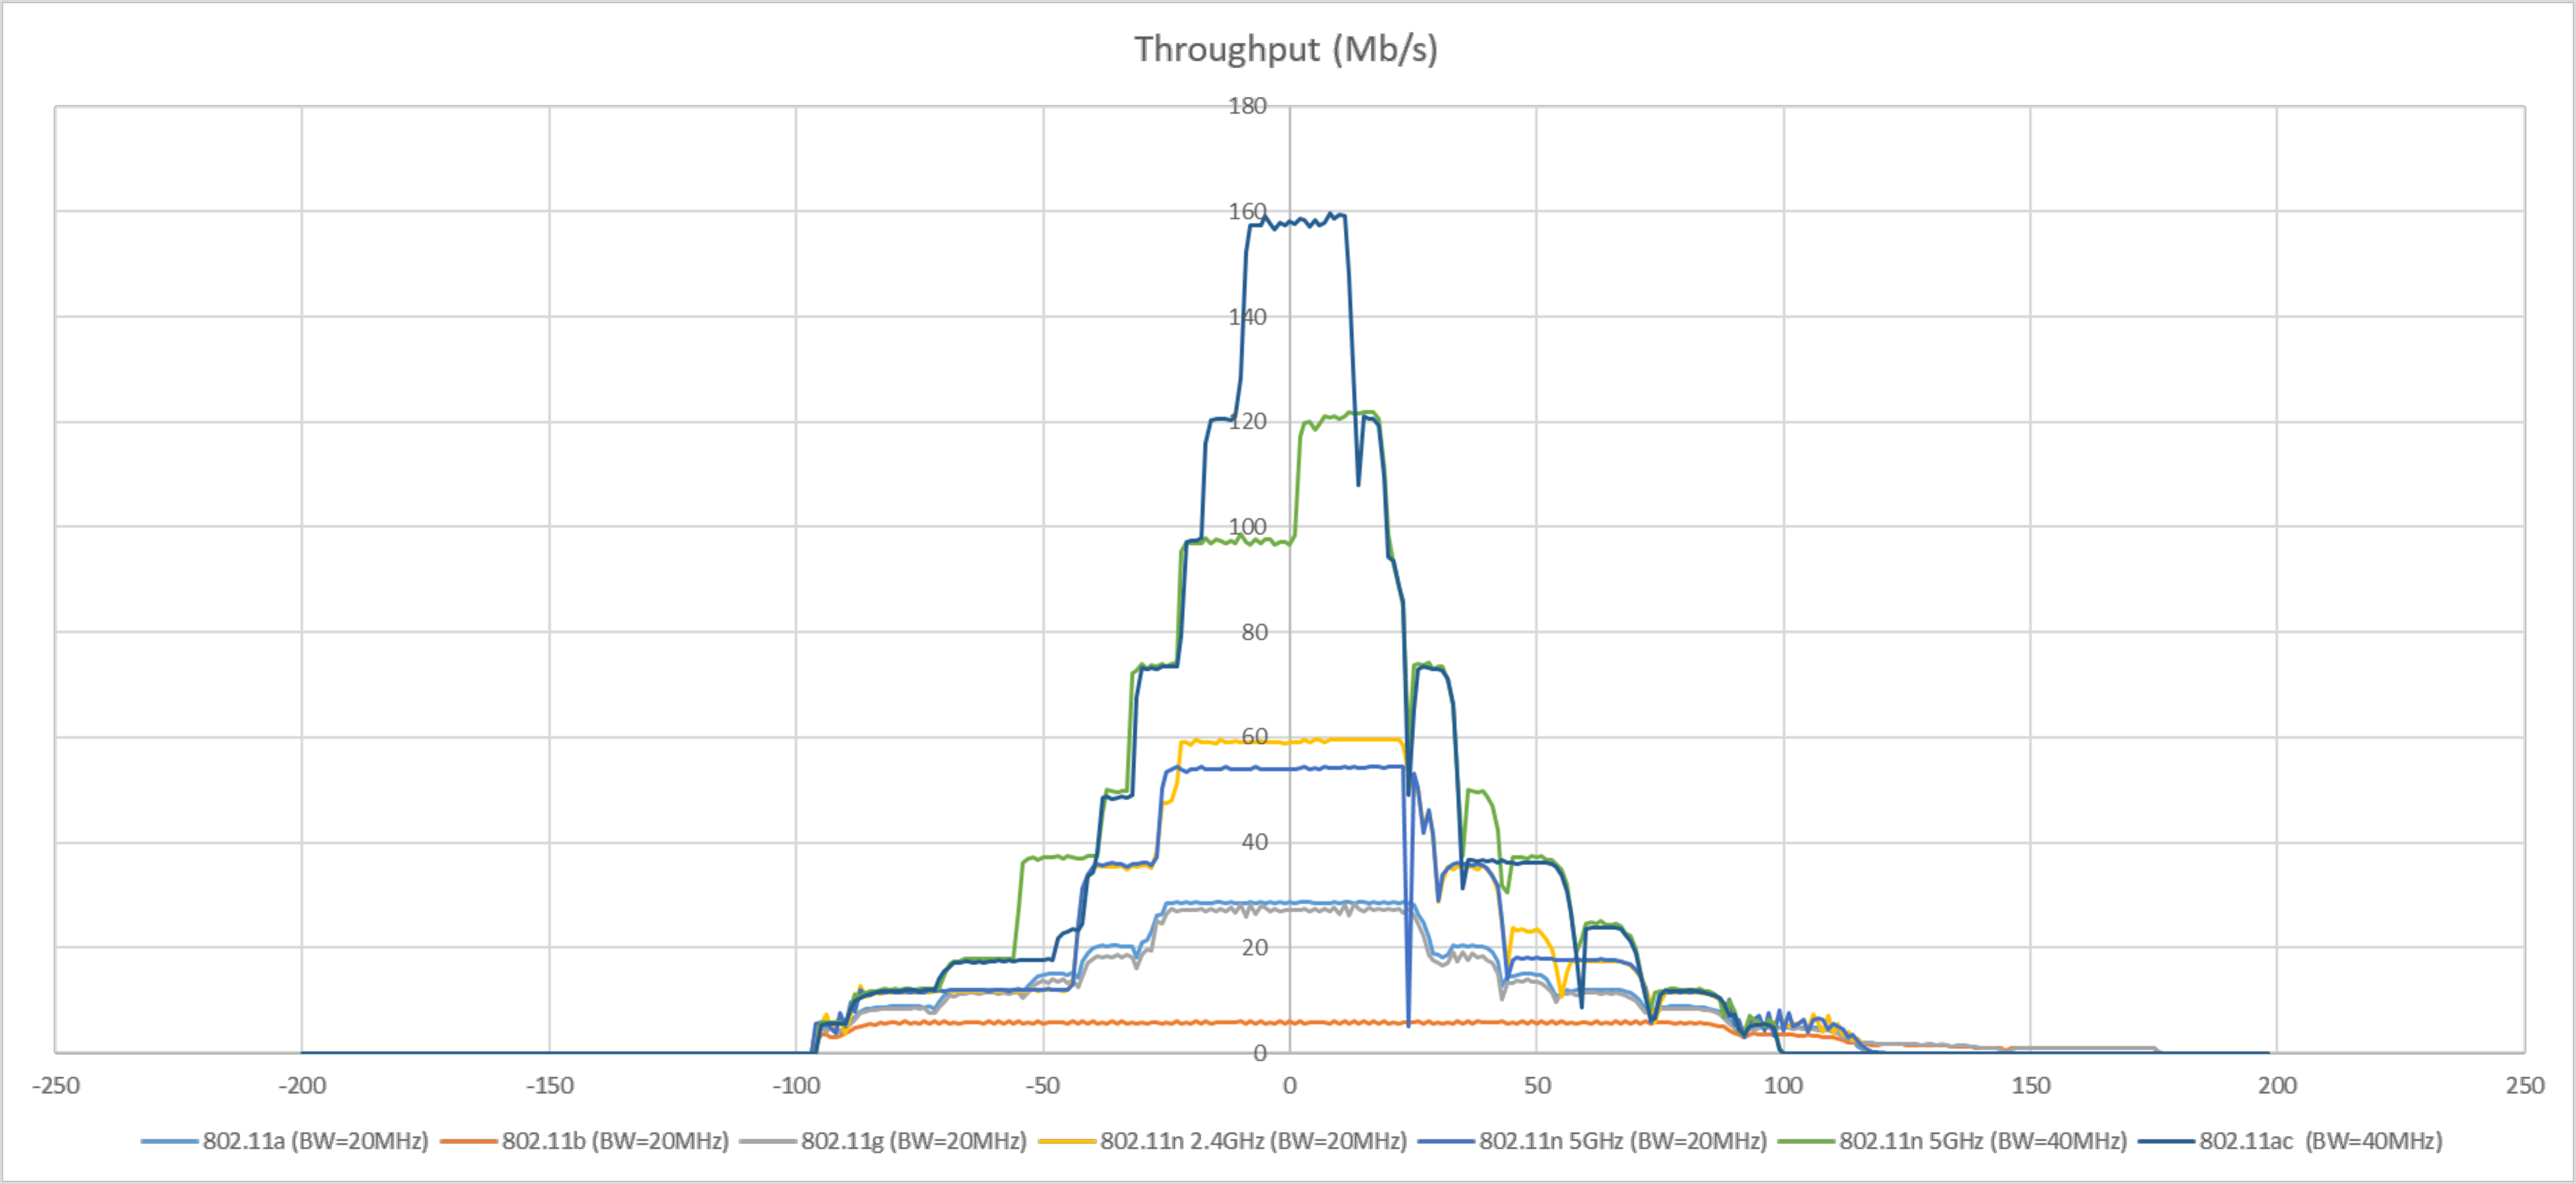
\includegraphics[width=\textwidth,keepaspectratio]{figures/50.PreliminaryW/distance-rate}
	\caption{Evaluation of moving node for different 802.11 network standards.}
	\label{fig:5.distance-rate}
\end{figure}


\subsection{Conclusions and future work}

	With this preliminary work, a first approach to create a communication scenario was presented. 
	The case study for this scenario was a set of moving trains in Porto-Caíde railway line, each of them with a constant speed of 12m/s (calculated to comply with the timetable) and scheduled to departure from origin station 10 minutes apart.
	
	With the OMNeT++ simulator, this scenario was simulated. Future work will comply with the variable speed of trains, with the consideration of stopping in stations. The expected output will be, for each existing communication link, the distance at each time between a train and a stationary node. This allows further evaluation of the throughput using an adequate simulator.
	
	In the second part of this preliminary work, the scenario was set to be a moving node between two points at fixed speed and having a stationary node in the middle. This allows the evaluation of the throughput for different 802.11 standards. With the NS-3 simulator, this scenario was implemented and tested. The results prove that this preliminary work will support the throughput evaluation of each communication link between the train and every base stations near the railway line of case study.




\section{Evaluation of the non-intrusive voltage sensor}

	%A critical issue that can be identified is the 
	Measurement of voltage waveforms using a non-intrusive approach is a critical issue in this research plan. 
	Brunelly et al. (2016) presents a possible non-intrusive voltage measurement for energy meters, \cite{brunelli2016}.
	On their work, as authors best knowledge, there is no commercially available non-intrusive sensor for voltage measurement in low-voltage wires (230-400 VAC). 
	Despite that, some studies are proposed in the literature for extra/high-voltage monitoring systems based on a capacitive cell.
	
	Based on the solution of \cite{brunelli2016}, a voltage sensor was implemented and tested, as presented in figure \ref{fig:5.voltage_sensor}, with the equivalent circuit in \ref{fig:5.voltage_sensor_eq}. 
	
	
	
	\begin{figure}[h!]
		\centering
		\begin{minipage}{.45\textwidth}
			\centering
			%		\vspace{2.5em}
			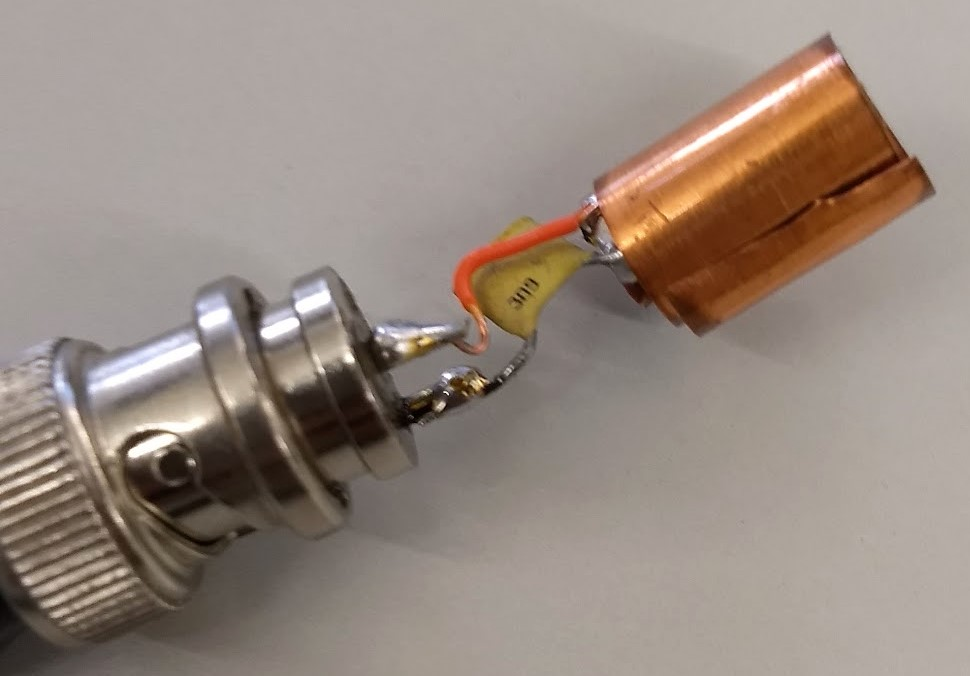
\includegraphics[width=0.7\textwidth,keepaspectratio]{figures/50.PreliminaryW/voltage_sensor}
			%		\vspace{2em}
			\captionof{figure}{Photo of implemented non-intrusive voltage sensor.}
			\label{fig:5.voltage_sensor}
		\end{minipage}%
		\begin{minipage}{.03\textwidth}  ~\end{minipage}	
		\begin{minipage}{.45\textwidth}
			\centering
			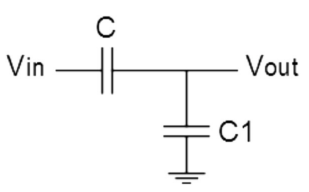
\includegraphics[width=0.8\textwidth,keepaspectratio]{figures/50.PreliminaryW/voltage_sensor_eq}
			%		\vspace{2em}
			\captionof{figure}{Equivalent circuit of non-intrusive voltage sensor.}
			\label{fig:5.voltage_sensor_eq}
		\end{minipage}
	\end{figure}

	
	To evaluate this sensor, two tests was performed: one with normal conditions of the grid, and other near a \ac{VSC}, respectively in figure \ref{fig:5.scope_0} and \ref{fig:5.scope_2}.
	
	
		\begin{figure}[h!]
		\centering
		\begin{minipage}{.45\textwidth}
			\centering
			%		\vspace{2.5em}
			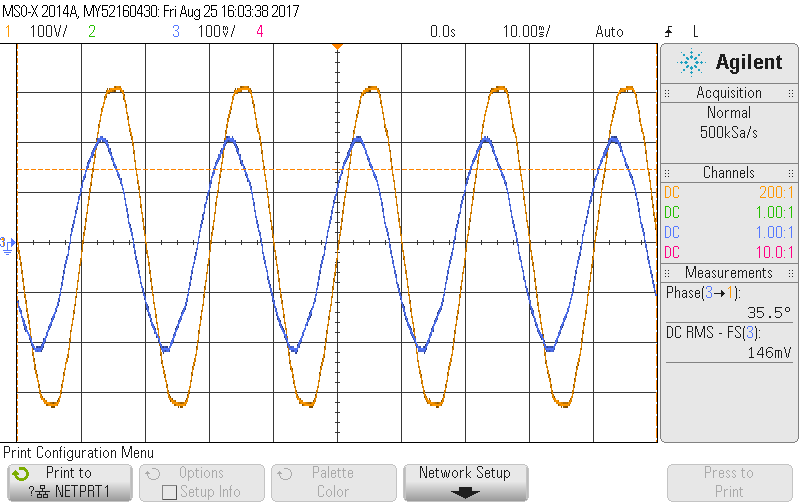
\includegraphics[width=\textwidth,keepaspectratio]{figures/50.PreliminaryW/scope_0}
			%		\vspace{2em}
			\captionof{figure}{Waveforms of acquired and sensed voltages in normal conditions: (orange) AC main voltage and (blue) voltage in sensor.}
			\label{fig:5.scope_0}
		\end{minipage}%
		\begin{minipage}{.03\textwidth}  ~\end{minipage}	
		\begin{minipage}{.45\textwidth}
			\centering
			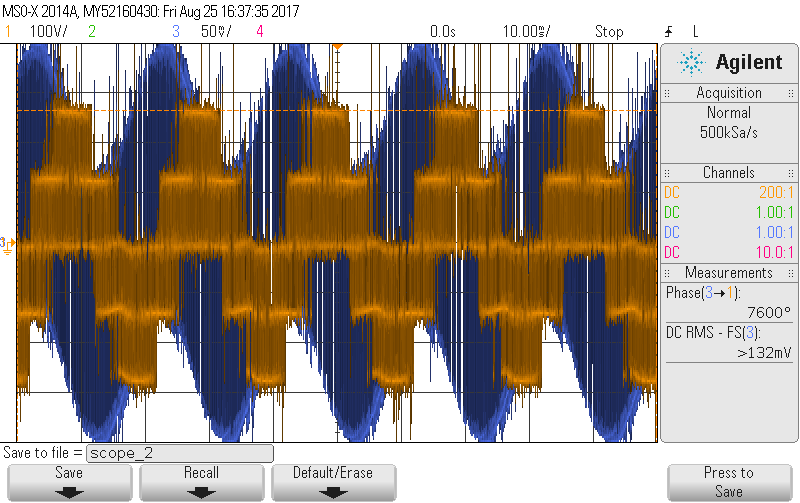
\includegraphics[width=\textwidth,keepaspectratio]{figures/50.PreliminaryW/scope_2}
			%		\vspace{2em}
			\captionof{figure}{Waveforms of acquired and sensed voltages in inverter: (orange) AC main voltage and (blue) voltage in sensor.}
			\label{fig:5.scope_2}
		\end{minipage}
	\end{figure}
	In ideal conditions, the voltage in the sensor is given by $V_{out} = (\frac{C}{C+C1})  V_{in} $.
	By having in consideration the impedance of the oscilloscope, the voltage in the sensor suffers a phase shift which is visible in both figures.
	In addition, with a combination of measurements and simulations, the values of C1 and C was obtained with a value of 3.9 nF and 3.2 pF respectively (considering that C1 is measured in the coaxial cable terminals and that the oscilloscope has a 1 M$\Omega$ and 11 pF equivalent internal circuit). 
	
	The \ac{VSC} is connected to the grid with a low-frequency transformer, which results in a line-to-line voltage of 200V (RMS) in the \ac{VSC}, \cite{martins2016}.

	The purpose of this preliminary work is to evaluate if this solution described in the state of the art is feasible to be implemented in an environment with huge amount of noise. At first evaluation the answer is negative, due to the need of extra work to estimate the voltage using the blue waveform of figure \ref{fig:5.scope_2}.
	
	
	Allowing the possibility to extract the voltage waveform, would be considered as a \textbf{contribution to the field of voltage measurement} in noisy environments, and in particular, in the railway environment.

	A second part of this preliminary work is the extraction of information from the sensor, in particular the phase of the voltage. To achieve this goal, a simple conditioning circuit made to amplify the voltage level of sensor to full range of $\mu$C ADC. The $\mu$C used was an Infineon XMC4500 and is responsible for the digital processing. In figure \ref{fig:5.generalArchitecture} is illustrated the architecture for signal conditioning and digital processing.
	
	\begin{figure}[h!]
		\centering
		\includegraphics[width=0.7\textwidth,keepaspectratio]{figures/50.PreliminaryW/generalArchitecture}
		\caption{Signal conditioning and digital processing architecture.}
		\label{fig:5.generalArchitecture}
	\end{figure}

	The digital processing is based on the flowchart of figure \ref{fig:5.processingArchitecture}.	
	The 50Hz digital filter is the first chain in the digital processing of the signal; the offset elimination algorithm finds the DC value of the input 50Hz signal and generates an output without offset. 
	The quadrature signal generation generates a signal with 20/4ms delay.
	
	\begin{figure}[h!]
		\centering
		\includegraphics[width=\textwidth,keepaspectratio]{figures/50.PreliminaryW/processingArchitecture}
		\caption{Digital processing structure.}
		\label{fig:5.processingArchitecture}
	\end{figure}

 
	
	The angle of the signal is then generated, as presented in figure \ref{fig:5.scope_9} where there is no phase compensation and the output of the phase estimation (in pink waveform) has a phase deviation around 10 degrees, compared with the line voltage (in orange waveform). In blue waveform is presented the estimated angle of voltage.
	
	In addition, in figure \ref{fig:5.scope_10}, the phase was compensated which resulted in an accurate estimation of the voltage phase, with a phase error around 1 degree.
	
	
	\begin{figure}[h!]
	\centering
	\begin{minipage}{.8\textwidth}
		\centering
		%		\vspace{2.5em}
		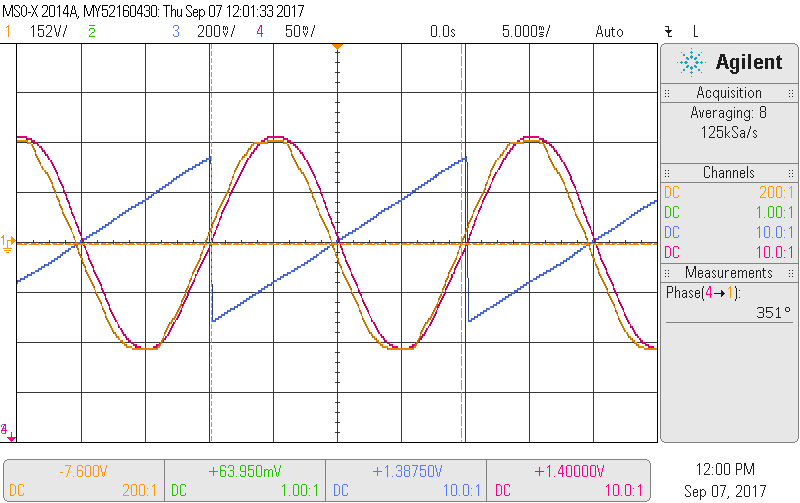
\includegraphics[width=0.8\textwidth,keepaspectratio]{figures/50.PreliminaryW/scope_9}
		%		\vspace{2em}
		\captionof{figure}{Waveforms of AC voltage (orange), estimated voltage (pink) and estimated phase angle (blue) without phase compensation.}
		\label{fig:5.scope_9}
	\end{minipage}%
	\begin{minipage}{.03\textwidth}  ~\end{minipage}	
	\begin{minipage}{.8\textwidth}
		\centering
		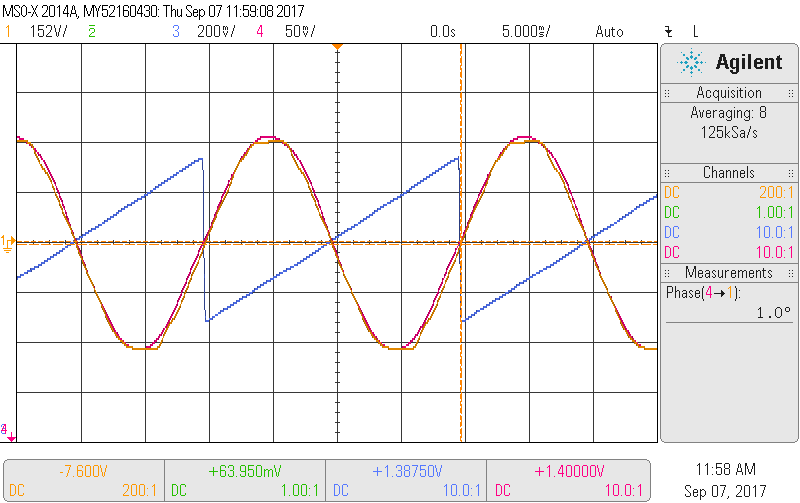
\includegraphics[width=0.8\textwidth,keepaspectratio]{figures/50.PreliminaryW/scope_10}
		%		\vspace{2em}
		\captionof{figure}{Waveforms of AC voltage (orange), estimated voltage (pink) and estimated phase angle (blue) with phase compensation.}
		\label{fig:5.scope_10}
	\end{minipage}
\end{figure}

	%Therefore and as previously presented in the second part of the methodology, the future work will start with the simulation of the electric field in a wire subjected to a VSC and the implementation of a solution that extracts the "real" voltage from the signal of the voltage sensor.
	
\subsection{Conclusions and future work}
	The work referred in literature that support these experimental results is feasible. \textbf{The voltage phase can be estimated with accuracy of around 1 degree};
	
	For future work, the following steps are identified:
	
	\begin{itemize}
		\setlength\itemsep{0em}
	
		\item The conditioning signal must support the dynamics of the switching frequency of the VSC. In one way, the bandwidth of the conditioning circuit must support the switching frequency dynamics; Complementarily, this conditioning circuit must adapt the voltage, using a programmable gain and offset amplifier, to better use the full-scale of the ADC.
		
		\item The execution time was measured and is around 50\% of the total available execution time (of 100us). Future work will promote the optimization of the time execution.
		
	%	\item In the estimated angle, an oscillation is visible. Since the grid frequency is stable at 50Hz, the estimated angle should not have that oscillation. Therefore, a filtering mechanism must be considered for the sawtooth waveform of the grid angle. An alternative solution will be the usage of a PLL. 
		
		\item Further future work will be the estimation of the voltage angle (of fundamental harmonic) of a VSC connected to a low-frequency transformer. The methodology to fulfill this estimation must be evaluated.
		
		\item As presented previously in the methodology chapter, the simulation of the sensor module must be performed to evaluate the application of this sensor to the train environment.
	\end{itemize}
